\chapter{Validation in Theta}
\section{Overview}
As mention: in the tetha specification.
"Theta is a generic, modular and configurable model checking framework developed at the Critical Systems Research Group of Budapest University of Technology and Economics, aiming to support the design and evaluation of abstraction refinement-based algorithms for the reachability analysis of various formalisms."
The way the Validator for witness 2.0 was implented in Theta is using XCFAs and Product Automaton. Even though 
XCFA's was chosen as formalism for further extensibility in the current version of the validator only the CFA
capabilities where used. For te moment the validator only supports Violation Witnesss. The way the violation
witness verifier works is described in the scheme below.

\begin{figure}[h]
    \centering
    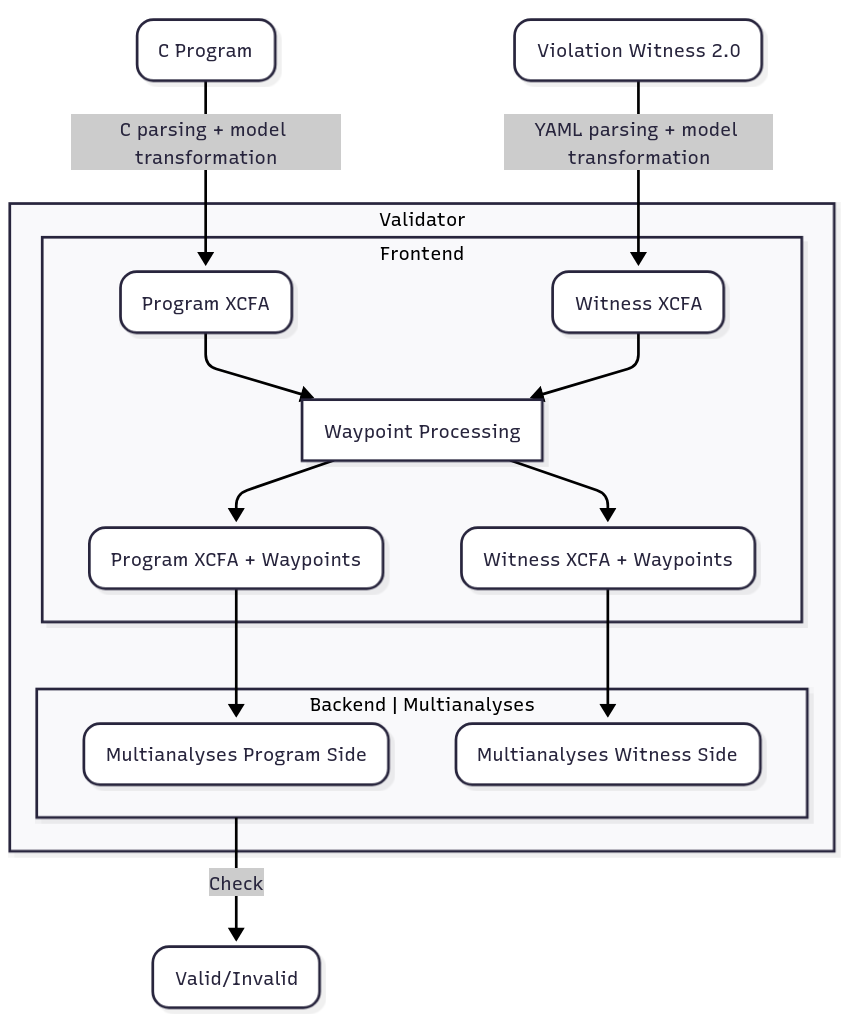
\includegraphics[width=0.8\textwidth]{figures/thetaValidator.png}
    \caption{Validation overview in Theta}
    \label{fig:Validation in Theta}
\end{figure}

% ---
% config:
%       theme: redux
% ---
% flowchart TD
%     cprogram("C Program")
%     witness("Violation Witness 2.0")
    
%     subgraph verifier["Validator"]
%         subgraph frontend["Frontend"]
%             programXCFA("Program XCFA")
%             witnessXCFA("Witness XCFA")
%             subgraph waypointProcessing["Waypoint Processing"]
%             end
%             programXCFAWay("Program XCFA + Waypoints")
%             witnessXCFAWay("Witness XCFA + Waypoints")
%         end
        
%         subgraph backend["Backend | Multianalyses"]
%             multiProgram("Multianalyses Program Side")
%             multiWitness("Multianalyses Witness Side")
%         end
%     end
    
%     output("Valid/Invalid")
    
%     cprogram -->|"C parsing + model transformation"| programXCFA
%     witness -->|"YAML parsing + model transformation"| witnessXCFA
%     programXCFA --> waypointProcessing
%     witnessXCFA --> waypointProcessing
%     waypointProcessing --> programXCFAWay
%     waypointProcessing --> witnessXCFAWay
%     programXCFAWay --> multiProgram
%     witnessXCFAWay --> multiWitness
%     backend -->|"Check"| output


There is no specification (and thus no specific safety property), because for the 
violation witness we are checking the reachability property—whether the error location
in the program and the target location in the witness are reached. The target location
of the witness is modeled as an error state to make the algorithm easy compatible with Multianalyses.

The C program is parsed and transformed into the program XCFA. The witness is parsed as YAML and 
then transformed into the witness XCFA. The violation witness can include waypoints of type avoid. 
In XCFA, a single trap node is created that all avoid waypoints point to. This works because the 
trap node (not connected to any other node) traps the execution of the violation witness, which 
means the error state of this witness cannot be reached.

While transforming the C program from AST to XCFA, much of the AST node data is added as metadata 
to the XCFA locations and edges. This metadata is used to ensure that the waypoints of the witness 
point to the correct places in the program XCFA. The pointing and correlation between the XCFAs are 
done using a global variable waypoint, which is assigned in the program XCFA and assumed in the 
witness XCFA.

From each XCFA, a Multianalysis side is created. Then the sides are combined to form the Multianalysis. 
Because of how the waypoint variable is handled, the Multianalysis is straightforward: each side 
is moved in sequence, starting from the program XCFA, until error states are reached in both XCFAs.

If both error states are reached, the witness is considered valid; otherwise, it is considered invalid.

\section{Generating XCFA from Violation Witnesses}
Within the validator in Theta, a crucial step involves transforming Violation Witnesses 
from their YAML into a more formal structure, specifically XCFA.

To facilitate this conversion, we need a clear methodology for translating each waypoint into 
its corresponding XCFA elements. Below, for every waypoint type, we'll outline how it's translated into 
the corresponding elements of the XCFA.
For our current purposes, it is sufficient to consider a waypoint (\texttt{wp}) variable as directly corresponding 
to a specific location in the C source file. The XCFA program itself also identifies these locations. 
Accordingly, each time the XCFA program arrives at one of these points, the XCFA witness
is called to process the same location. 
In our specific case, since the waypoints for the witness are essentially edges, the \texttt{wp} 
variable role is simply to determine which particular edge needs to be checked.

We consider two types of assumption waypoints:
\begin{itemize}
  \item An \textbf{avoid assumption} specifies a condition that the program must 
    \textit{not} satisfy. In other words, this assumption must not be met.
    An avoid assumption can be thought of as a negated follow assumption that 
    does not cause an advancement to the next segment.
    This implies that each time the program logic encounters an avoid assumption, 
    it must check that the specified condition does not hold.
    If the condition does not hold (i.e., the avoidance is successful), the program can 
    be modeled as having an edge transitioning back to, or remaining within, the current segment node.
    Conversely, if the condition \emph{does} hold (i.e., the program is unsuccessful in avoiding it), 
    then the execution will have no further states to transition to.
  \item A \textbf{follow assumption} dictates that the program \textit{must} 
    traverse a specific waypoint within the current segment.
    After successfully passing through this waypoint, the program is required to transition 
    to the next segment. This means the waypoint associated with a \textbf{follow} assumption 
    must be visited only once.
    Therefore, this type of assumption is represented by an edge leading from the current 
    state (after satisfying the waypoint condition) to the node representing the subsequent segment.
\end{itemize}

\begin{figure}[htbp]
  \centering
  \begin{minipage}[t]{0.25\textwidth}
    \begin{lstlisting}[style=c, columns=flexibl]
- segment:
  - waypoint:
    type: "assumption"
    action: "avoid"
    constraint: <C_1>
    location: <wp_1>
  - waypoint:
    type: "assumption"
    action: "avoid"
    constraint: <C_2>
    location: <wp_2>
  - waypoint:
    type: "assumption"
    action: "follow"
    constraint: <C_3>
    location: <wp_3>
    \end{lstlisting}
    \end{minipage}
    \begin{tikzpicture}[
        baseline=(current bounding box.north),
        node distance=2cm,
        >={Stealth[scale=1.2]},
        every edge/.style={draw, ->},
        solidnode/.style={draw, circle, minimum size=1.2cm}, % Solid nodes
        dashednode/.style={draw, dashed, circle, minimum size=1.2cm} % Dashed nodes
    ]

    \node[dashednode] (SN1) {$s_{n-1}$};
    \node[solidnode, below=1cm of SN1] (SN) {$s_n$};
    \node[dashednode, below=1cm of SN] (SN2) {$s_{n+1}$};

    \path (SN1) edge[dashed] (SN)
        (SN) edge[out=150, in=210, min distance=1.2cm] node[left, font=\scriptsize] {$\neg C_1 \land \text{wp} = wp_1$} (SN)
        (SN) edge[out=150, in=210, min distance=5cm] node[left, font=\scriptsize] {$\neg C_2 \land \text{wp} = wp_2$} (SN)
        (SN) edge[out=30, in=-30, min distance=1.2cm] node[right, font=\scriptsize, align=left] {%
          $\text{wp} < wp_1 \lor$ \\
          $\text{wp} > wp_3$%
        } (SN)
        (SN) edge node[midway, right, font=\scriptsize] {$C_3 \land \text{wp} = wp_3$} (SN2);

    \end{tikzpicture}
  \caption{XCFA mapping of the assumtion type waypoints and their constrains. The \texttt{C}
  variables are c expressions and the \texttt{wp} variables are just a tuple of row:col.}
  \label{fig:combined}
\end{figure}

One of the edges depicted in the figure, which has not been previously explained, is the loop at 
state $S_n$. This loop is labeled with the condition $\texttt{wp} < wp_1 \lor \texttt{wp} > wp_3$. Such 
an edge, which we will call the \textbf{segment guard} edge, is necessary because, within the current 
segment, we are only concerned with processing waypoints that specifically correspond to this segment. 
Since the waypoints are ordered according to their \texttt{wp} value (these are values mapped from their 
source code locations, rather than the locations themselves, which means that even if the source locations 
are not ordered, the \texttt{wp} values are), a range check, as exemplified by the aforementioned label, 
is sufficient.

A while loop provides a good example for understanding the difference between 
\emph{avoid} and \emph{follow} assumptions.
To clarify the usual confusion surrounding these concepts, and to explain why they 
are necessary and defined in this manner, consider the following illustration.
Suppose, looking at the simple \texttt{while} loop in Figure~3.3, the objective is 
to ensure tha the variable $v$ always remains greater than 200; effectively, this means 
we aim for the $s$ variable to overflow.
One could achieve this by employing a \emph{follow} assumption, such as $v > 200$, 
applied across n distinct program segments.
Alternatively, a more concise approach is to define a single \emph{avoid} 
assumption for the relevant segment, for instance, to avoid paths where $v \le 200$.

\begin{figure}[H]
  \centering
  \begin{minipage}[t]{0.40\textwidth}
    \begin{lstlisting}[style=c]
uchar v=0, s=0, i=0, n=2;
while (i < n) {
  v = nondet(); 
  // AVOID (assume v <= 200)
  s += v; ++i;
}\end{lstlisting}
  \end{minipage}
  \begin{tikzpicture}[
      baseline=(current bounding box.north),
      node distance=1.6cm,
      >={Stealth[scale=1.0]},
      every edge/.style={draw, ->},
      solidnode/.style={draw, circle, minimum size=0.8cm},
      dashednode/.style={draw, dashed, circle, minimum size=0.8cm},
      scale=1,
      transform shape
  ]

  % Nodes
  \node[solidnode] (loop_start) {$\ell_0$};
  \node[solidnode, below of=loop_start] (main_path) {$\ell_1$};
  \node[solidnode, right of=loop_start] (alternative) {$\ell_1$};

  % Incoming dashed arrow (added as requested)
  \node[left of=loop_start, xshift=-0.5cm] (incoming) {};
  \draw[dashed, ->] (incoming) -- node[above] {entry} (loop_start);

  % Transitions
  \path 
      (loop_start) edge node[right, font=\scriptsize] {$i < n$} (main_path)
      (loop_start) edge node[above, font=\scriptsize] {$i \geq n$} (alternative)
      (main_path) edge[bend left=50] node[left, font=\scriptsize] {$\begin{array}{l}
                                   v := nondet()\\ 
                                   s := s + v\\
                                   i := i + 1
                                   \end{array}$} (loop_start);

  % Outgoing dashed arrow (added as requested)
  \node[right of=alternative, xshift=0.5cm] (outgoing) {};
  \draw[dashed, ->] (alternative) -- node[above] {exit} (outgoing);

  \end{tikzpicture}

  \caption{A Simple Whileloop and its corresponding branching in the XCFA of the program.}
  \label{fig:combined}
\end{figure}

Branching waypoints can be located at control flow statements such as \texttt{if}, \texttt{while}, a 
\texttt{ternary operator (?:)}, or a \texttt{switch} statement.
It is important to first note that in an XCFA, these C constructs are all represented as branching structures.
The XCFA representation for \texttt{if}, \texttt{while} statements and the \texttt{ternary operator (?:)} is generally 
similar, whereas it tends to be more complex for \texttt{switch} statements.
As an illustration, Figure~3.3 depicts the XCFA of a \texttt{while} loop, where the XCFA branches into two directions. 
A \texttt{switch} statement, in contrast, typically involves a greater number of branches.
This branching mechanism enables the differentiation of the path taken within the XCFA program 
solely by using the \texttt{wp} variable.
For example, if a branching waypoint indicates that the \texttt{while} loop condition evaluates to true,
the \texttt{wp} variable for that waypoint would be mapped to the edge between $\ell_0$ and $\ell_1$. 
Consequently, if the XCFA program follows the path corresponding to the condition $i>n$ (representing 
the 'true' branch in this scenario), we can determine that this specific branch was taken by inspecting 
the \texttt{wp} variable.



In the current version of Theta's validator, we only support \texttt{if} and \texttt{while} types of branching waypoints:
\begin{itemize}
  \item An \textbf{avoid branching} waypoint dictates that the program execution should never 
    traverse the branch specified by this waypoint. In other words, the \texttt{wp} variable 
    should never be equal to (i.e., point to) the location associated with this type of waypoint.
    To represent this in the witness XCFA, no specific action is taken; essentially, no edge is defined 
    for this type of waypoint. This is because encountering this type of waypoint signifies that the
    program execution should halt (i.e., "get stuck").
    This approach differs from the previously discussed \texttt{avoid assumption}. In the case of an 
    \texttt{avoid assumption}, even if the \texttt{wp} variable aligns with the waypoint's location, 
    the execution can still proceed if the associated constraint does not hold.
    However, for the type of waypoint being discussed here, encountering it mandates an immediate stop of the execution.
    This is achieved in the witness XCFA by not adding an edge, effectively meaning there is no subsequent state to transition to.
  \item A \textbf{follow branching} waypoint indicates that the program execution \emph{must} 
    follow this particular branch. We can easily verify if the program indeed followed this
    branch by checking if the \texttt{wp} variable is equal to the location of this waypoint. 
    In the witness XCFA, this can be represented by an edge leading to the subsequent segment, which is
    traversed if the \texttt{wp} variable matches this waypoint's location.
\end{itemize}

It should be noted that branching waypoints possess a constraint indicating how the condition of an \texttt{if}, \texttt{while}, 
\texttt{ternary operator (?:)}, or \texttt{switch} statement evaluated.
For \texttt{if}, \texttt{while}, and the \texttt{ternary operator (?:)}, this evaluation can result in "true" or "false".
For a \texttt{switch} statement, it can be an integer constant (representing the value of the variable being switched upon) or the "default" case.
Consequently, this constraint informs us which path the program should take.
Since the \texttt{wp} variable is associated with the path we intend the program to follow, this implies that the \texttt{wp}
variable also implicitly "contains" this constraint (i.e., the constraint can be inferred from it).
Therefore, in a potentially simplified YAML witness representation (such as one discussed below), the explicit constraint might 
be omitted, with only the location being kept. This, however, is not the case in the complete or actual YAML witness specification.


\begin{figure}[H]
  \centering
  \begin{minipage}[t]{0.35\textwidth}
    \begin{lstlisting}[style=c, columns=flexibl]
    - segment:
      - waypoint:
        type: "branching"
        action: "avoid"
        location: <wp_1>
      - waypoint:
        type: "branching"
        action: "avoid"
        location: <wp_2>
      - waypoint:
        type: "branching"
        action: "follow"
        location: <wp_3>
    \end{lstlisting}
    \end{minipage}
    \hspace{2cm}
    \begin{tikzpicture}[
        baseline=(current bounding box.north),
        node distance=2cm,
        >={Stealth[scale=1.2]},
        every edge/.style={draw, ->},
        solidnode/.style={draw, circle, minimum size=1.2cm}, % Solid nodes
        dashednode/.style={draw, dashed, circle, minimum size=1.2cm} % Dashed nodes
    ]

    \node[dashednode] (SN1) {$s_{n-1}$};
    \node[solidnode, below=1cm of SN1] (SN) {$s_n$};
    \node[dashednode, below=1cm of SN] (SN2) {$s_{n+1}$};

    \path (SN1) edge[dashed] (SN)
        (SN) edge[out=30, in=-30, min distance=1.2cm] node[right, font=\scriptsize, align=left] {%
          $\text{wp} < wp_1 \lor$ \\
          $\text{wp} > wp_3$%
        } (SN)
        (SN) edge node[midway, right] {$\text{wp} = wp_3$} (SN2); 

    \end{tikzpicture}
  \caption{XCFA mapping of a branching-type waypoint, where the \texttt{wp} variable is a tuple (row:col, constraint)
  indicating which XCFA branch was taken.}
  \label{fig:combined}
\end{figure}

There is only one type of target waypoint:
\begin{itemize}
  \item A \textbf{follow target} waypoint indicates that the program execution should reach 
    the designated error location. It is positioned immediately before the error, 
    ensuring that no other program evaluations occur before the error state is encountered. 
    In the witness XCFA, this can be readily represented by an edge pointing directly to the error location.
\end{itemize}
This type of waypoint does not have an associated constraint.

\begin{figure}[H]
  \centering
  \begin{minipage}[t]{0.35\textwidth}
    \begin{lstlisting}[style=c, columns=flexibl]
    - segment:
      - waypoint:
        type: "target"
        action: "follow"
        location: <wp_0>
    \end{lstlisting}
    \end{minipage}
    \hspace{2cm}
    \begin{tikzpicture}[
        baseline=(current bounding box.north),
        node distance=2cm,
        >={Stealth[scale=1.2]},
        every edge/.style={draw, ->},
        solidnode/.style={draw, circle, minimum size=1.2cm}, % Solid nodes
        dashednode/.style={draw, dashed, circle, minimum size=1.2cm}, % Dashed nodes
        errornode/.style={solidnode, fill=red!20}
    ]

    \node[dashednode] (SN1) {$s_{n-1}$};
    \node[solidnode, below=1cm of SN1] (SN) {$s_n$};
    \node[errornode, below=1cm of SN] (SN2) {error};

    \path (SN1) edge[dashed] (SN)
        (SN) edge[out=30, in=-30, min distance=1.2cm] node[right, font=\scriptsize, align=left] {%
          $\text{wp} < wp_0 \lor$ \\
          $\text{wp} > wp_0$%
        } (SN)
        (SN) edge node[midway, right] {$\text{wp} = wp_0$} (SN2); 

    \end{tikzpicture}
  \caption{XCFA mapping of target type waypoint. The \texttt{wp} variables are a tuple of row:col.}
  \label{fig:combined}
\end{figure}


A segment is designated as final if its follow waypoint is a target.
The following is an example segment that includes all the aforementioned types of waypoints.

\begin{figure}[H]
  \centering
  \begin{minipage}[t]{0.35\textwidth}
    \begin{lstlisting}[style=c, columns=flexibl]
    - segment:
      - waypoint:
        type: "branching"
        action: "avoid"
        location: <wp_1>
      - waypoint:
        type: "assumption"
        action: "avoid"
        constraint: <C_2>
        location: <wp_2>
      - waypoint:
        type: "target"
        action: "follow"
        location: <wp_3>
    \end{lstlisting}
    \end{minipage}
    \begin{tikzpicture}[
        baseline=(current bounding box.north),
        node distance=2cm,
        >={Stealth[scale=1.2]},
        every edge/.style={draw, ->},
        solidnode/.style={draw, circle, minimum size=1.2cm}, % Solid nodes
        dashednode/.style={draw, dashed, circle, minimum size=1.2cm} % Dashed nodes
    ]

    \node[dashednode] (SN1) {$s_{n-1}$};
    \node[solidnode, below=1cm of SN1] (SN) {$s_n$};
    \node[dashednode, below=1cm of SN] (SN2) {$s_{n+1}$};

    \path (SN1) edge[dashed] (SN)
        (SN) edge[out=150, in=210, min distance=1.2cm] node[left, font=\scriptsize] {$\neg C_2 \land \text{wp} = wp_2$} (SN)
        (SN) edge[out=30, in=-30, min distance=1.2cm] node[right, font=\scriptsize, align=left] {%
          $\text{wp} < wp_1 \lor$ \\
          $\text{wp} > wp_3$%
        } (SN)
        (SN) edge node[midway, right] {$\text{wp} = wp{}_3$} (SN2); 

    \end{tikzpicture}
  \caption{XCFA mapping of a final segment containing branching, assumption, and target waypoints, along with their respective constraints.}
  \label{fig:combined}
\end{figure}


\section{Combining and Executing the XCFA's}
As seen in Figure~3.1, after the program and witness XCFAs are created and their 
corresponding waypoints (locations) are matched, we proceed to run the Multianalysis. 
Before explaining how the XCFAs are executed together, we should first examine what 
a generic witness may look like. Figure~3.7 (left) shows such a witness.

A witness XCFA can be composed of a start location, a sequence of one or more segments, and 
an error location. Segments are represented by nodes labeled $S_i$.
To represent the possibility of many segments, nodes such as $S_{n-1}$ and $S_{n+1}$ are visualized as dashed (meaning optional).
From the discussion above, it becomes clear that segment $S_n$ is a depiction of a general segment.
Dashed edges signify that they may or may not be present. For instance, several dashed edges on 
the right side indicate that there can be multiple \texttt{avoid} conditions within a segment. 
In contrast, the bold edges, which represent the \texttt{follow} waypoint and the segment guard, 
are necessary components.
Here, the range $1 < i \le n-1$ for an index $i$ delineates the waypoints within the current segment 
$S_n$, excluding the final one; these waypoints are labeled $wp_{s_{ni}}$.
The \texttt{C} variables in this context represent several expressions combined. They can aslo be empty.


On the right, a representation of a generic program XCFA is shown.
Here, \texttt{k} within the program XCFA represents the branching number. 
For an \texttt{if} statement, this number is 2, whereas for a \texttt{switch} statement, 
it can be as large as the number of cases in the switch.
It is important to note that not all edges in this XCFA necessarily have associated waypoints.
The bold edge depicted between $\ell_n$ and $\ell_{n+1}$ represents 
an arbitrary edge within the program XCFA that does have an associated waypoint.

\begin{figure}[htbp]
  \centering
  \begin{minipage}[t]{0.35\textwidth}
    \begin{tikzpicture}[
        baseline=(current bounding box.north),
        node distance=2cm,
        >={Stealth[scale=1.2]},
        every edge/.style={draw, ->},
        solidnode/.style={draw, circle, minimum size=1.2cm},
        dashednode/.style={draw, dashed, circle, minimum size=1.2cm},
        startnode/.style={solidnode, fill=black!20},
        errornode/.style={solidnode, fill=red!20}
    ]

    % Nodes
    \node[startnode] (start) {start};
    \node[dashednode, below=1cm of start] (SN1) {$s_{n-1}$};
    \node[solidnode, below=1cm of SN1] (SN) {$s_n$};
    \node[dashednode, below=1cm of SN] (SN2) {$s_{n+1}$};
    \node[errornode, below=1cm of SN2] (error) {error};

    % Edges
    \draw[dashed, dotted] (start) -- (SN1); % Dotted-dashed entry
    \path (SN1) edge[dashed] (SN)
        (SN) edge[dashed, out=150, in=210, min distance=1.2cm] node[left, font=\scriptsize, align=left] {%
            [$\neg C_i \land$ \\
            $\text{wp} = wp_{s_ni}$] \\
            $\text{run} := \text{false}$%
        } (SN)
        (SN) edge[dashed, out=150, in=210, min distance=3cm] (SN)
        (SN) edge[out=30, in=-30, min distance=1.2cm] node[right, font=\scriptsize, align=left] {%
           [$\text{wp} < wp_{s_n1} \lor$ \\
            $\text{wp} > wp_{s_nn}$] \\
            $\text{run} := \text{false}$%
        } (SN)
        (SN) edge node[midway, right, font=\scriptsize, align=left] {%
           [$\neg C_n \land$ \\
            $\text{wp} = wp_{s_nn}$] \\
            $\text{run} := \text{false}$%
        } (SN2);
    \draw[dashed, dotted] (SN2) -- (error);

    % Additional dashed edges
    \draw[dashed] (SN1) edge[out=150,in=210,looseness=4] (SN1); % Self-loop
    % \draw[dashed] (SN1) edge[out=150,in=210,looseness=7] (SN1); % Self-loop
    % \draw[dashed] (SN1) edge[out=30,in=-30, looseness=4] (SN1); % Self-loop
    \draw[dashed] (SN2) edge[out=150,in=210, looseness=4] (SN2); % Self-loop
    % \draw[dashed] (SN2) edge[out=150,in=210, looseness=7] (SN2); % Self-loop
    % \draw[dashed] (SN2) edge[out=30,in=-30, looseness=4] (SN2); % Self-loop

    \end{tikzpicture}
  \end{minipage}
  \hspace{2cm}
  \begin{tikzpicture}[
      baseline=(current bounding box.north),
      node distance=2cm,
      >={Stealth[scale=1.2]},
      every edge/.style={draw, ->},
      solidnode/.style={draw, circle, minimum size=1.2cm},
      dashednode/.style={draw, dashed, circle, minimum size=1.2cm},
      startnode/.style={solidnode, fill=black!20},
      errornode/.style={solidnode, fill=red!20}
  ]

  % Nodes
  \node[startnode] (start) {start};
  \node[dashednode, below=1cm of start] (L1) {$l_{n-1}$};
  \node[solidnode, below=1cm of L1] (L) {$l_n$};
  \node[dashednode, below=1cm of L] (L2) {$l_{n+1}$};
  \node[dashednode, below=1cm of L, left=1 cm of L2] (Lk) {$l_{n+k}$};
  \node[errornode, below=1cm of L2] (error) {error};

  % Edges
  \draw[dashed, dotted] (start) -- (L1); % Dotted-dashed entry
  \path (L1) edge[dashed] (L)
      (L) edge node[left, right,font=\scriptsize, align=left] {%
        [$\neg exp_n$] \\
            $\text{wp} := wp_{s_ni}$ \\
            $\text{run} := \text{true}$%
        } (L2)
      (L2) edge[dashed, out=30, in=-30] (L)
      (L) edge[dashed]  (Lk)
      (Lk) edge[dashed, out=70, in=185]  (L);

  \draw[dashed, dotted] (L2) -- (error);
  \draw[dashed, dotted] (Lk) -- (error);

  % Additional dashed edges
  % \draw[dashed] (L1) to[out=150,in=210,looseness=4] (L1); % Self-loop
  % \draw[dashed] (L2) to[out=150,in=210,looseness=4] (L2); % Self-loop
  % \draw[dashed] (Lk) to[out=150,in=210,looseness=4] (Lk); % Self-loop

  \end{tikzpicture}
\caption{Comparison of a generic witness XCFA (left) and a generic program 
XCFA (right). Dashed nodes or edges are optional. Dotted lines represent an 
abstracted list of segments. Each XCFA has a start and an error location.}
  \label{fig:combined}
\end{figure}

Now, let's discuss how the multi-analysis is run. We begin from the \texttt{start} node in both XCFAs. 
The program XCFA's execution proceeds until a waypoint is encountered. Suppose the current waypoint 
reached is $\texttt{wp}_{s_ni}$.
The \texttt{wp} variable is set to this current waypoint, $\texttt{wp}_{s_ni}$, and the \texttt{run}
variable is set to \texttt{true}, indicating that a waypoint has been processed and the witness XCFA 
should now execute. The $\texttt{run} := \texttt{true}$ assignment is associated with every waypoint
location in the program XCFA, while a $\texttt{run} := \texttt{false}$ assignment is present on every
edge of the witness XCFA. This detail was abstracted away previously, but here it can be clearly seen 
that every edge of the witness XCFA has the $\texttt{run} := \texttt{false}$ assignment.
Thus, after the \texttt{run} variable is set to \texttt{true} by the program XCFA, control transfers to the witness XCFA.



\textbf{The variables and the state are shared between the XCFAs}, so the witness XCFA utilizes the set
\texttt{wp} variable and the current program state to take one step.
The \texttt{wp} variable, in conjunction with edge guards, is used to determine which edge (and thus 
which waypoint) is currently being evaluated. The conditions of this chosen edge are then checked for satisfiability.
If the guard conditions on this edge are not met, the execution halts, and the witness is deemed invalid. 
Conversely, if the guard conditions are met, depending on the \texttt{wp} variable, the witness XCFA may 
either remain in the current segment or transition to the next one:
\begin{itemize}
    \item If \texttt{wp} does not correspond to a waypoint within the current segment, the segment 
      guard edge is taken, and the witness XCFA remains in the current segment.
    \item If \texttt{wp} corresponds to one of the \texttt{avoid} edges, the witness XCFA remains 
      in the current segment.
    \item If \texttt{wp} corresponds to the \texttt{follow} waypoint, the witness XCFA transitions 
      to the next segment.
\end{itemize}
After an edge in the witness XCFA is taken, the \texttt{run} variable is set to \texttt{false}, 
signaling that the program XCFA now resumes control of the execution.
This process continues until the error states of both XCFAs are reached simultaneously, at which point 
the witness is considered valid.

Even though one might intuitively consider the states of the program XCFA and the witness XCFA
separately, they are, in this context, components of product states within a unified product
automaton. The analysis method employed, termed multianalysis, operates directly on this
product automaton. The product states are pairs, denoted as $(s, l)$, where $s$ is a state from the
witness XCFA and $l$ is a state from the program XCFA. A set, which we will call
$\text{\texttt{states}}$, is maintained to hold the current product states being processed.
For traversing these product states, various strategies such as Breadth-First Search (BFS) or
Depth-First Search (DFS) can be employed. For this explanation, a BFS order will be adopted
due to its illustrative simplicity. However, it is worth noting that for the specific example
discussed below, the choice between BFS and DFS will not make a discernible difference in the
trace. This is because the set of current states, $\text{\texttt{states}}$, will consistently
contain only a single state. This is a consequence of the witness (in the example below, as not
every witness would necessarily provide such a narrow path) explicitly dictating which branch the
program must take at any decision point, thereby preventing the simultaneous exploration of
multiple paths.

The construction of edges in this product automaton is governed by the edges of the constituent XCFAs:
\begin{itemize}
    \item If an edge exists in the witness XCFA from state $s_i$ to $s_k$, then for any program XCFA
    state $l$, an edge is formed in the product automaton from the product state $(s_i, l)$ to $(s_k, l)$.
    \item Symmetrically, if an edge exists in the program XCFA from state $l_i$ to $l_k$, then for
    any witness XCFA state $s$, an edge is formed in the product automaton from
    the product state $(s, l_i)$ to $(s, l_k)$.
\end{itemize}

We also require a set to maintain the shared state, which we will call $\text{\texttt{varsExpl}}$.
For this example, we will employ an explicit analysis, meaning we track explicit variable values
rather than symbolic conditions, for simplicity.
The execution begins with $\text{\texttt{states}} = \{ (\text{start}_p, \text{start}_w) \}$ and
$\text{\texttt{varsExpl}} = \{ \}$.
Variables are initially undefined and will be set upon their first assignment.

Both XCFAs are positioned at their respective start nodes. Since $\text{\texttt{run}}$ is
initially $\text{\texttt{undefined}}$, by default the program XCFA proceeds first.

The core algorithmic process is relatively straightforward: the active XCFA is identified, its
permissible outgoing edges are determined, and these edges are then traversed to explore the states
reached. This transition can be represented by the set of $\text{edges\_taken}$ and the resulting
state. A single step of the algorithm can thus be thought of as:
\begin{lstlisting}[style=C, language=C]
||||| Step n |||||
edges_taken = {...}; // edges where the enabling condition evaluated to true
states = {...};        // resulting states of taking those edges
varsExpl = {...};    // the explicit shared state of variables belonging to the XCFAs.
\end{lstlisting}
These steps are run until the state $\text{\texttt{states}} = \{(\text{error}_p, \text{error}_w)\}$ is reached,
where $\text{error}_p$ is the error state of the program XCFA and $\text{error}_w$ is the error state of the
witness XCFA. If we manage to reach this state, it means we have successfully passed all the segments
and the waypoints in them.


\section{Example}
To clarify how the validator works, Figures~3.8 and~3.9 display an example of an unsafe C program 
and a corresponding violation witness for this program, along with their respective XCFAs.
In this context, the \texttt{nondet()} function returns a nondeterministic value within the \
range of 0 to 255, inclusive (i.e., the range of an \texttt{unsigned char}).

\begin{figure}[htbp]
  \centering
  \begin{minipage}[t]{0.35\textwidth}
\begin{lstlisting}[
    style=c,
    label=lst:code,
    numbers=left,
    firstnumber=1,
    numberstyle=\tiny\color{gray}
]
int main() {
  unsigned char n = nondet();
  if (n == 0) return 0; 

  unsigned char v = 0;
  unsigned char s = 0;
  unsigned int i = 0; 
  while (i < n) {
    v = nondet();
    s += v;
    ++i;
  } 

  if (s < v) { 
    reach_error(); 
    return 1; 
  }

  return 0;
}\end{lstlisting}
  \end{minipage}
  \hspace{1cm}
\begin{tikzpicture}[
    node distance=2cm,
    >={Stealth[scale=1.2]},
    baseline=(current bounding box.north),
    every edge/.style={draw, ->},
    solidnode/.style={draw, circle, minimum size=1.0cm},
    startnode/.style={solidnode, fill=black!20},
    errornode/.style={solidnode, fill=red!20},
    retnode/.style={solidnode, fill=green!20},
    font=\scriptsize
]

% Main nodes
\node[startnode] (l0) {$\text{start}$};
\node[solidnode, below of=l0] (l1) {$\ell_1$};
\node[retnode, below left=1.5cm of l1] (ret0) {ret};
\node[solidnode, below right=1.5cm of l1] (l2) {$\ell_2$};
\node[solidnode, below of=l2] (l3) {$\ell_3$};
\node[solidnode, left of=l3, node distance=3cm] (l4) {$\ell_4$};
\node[solidnode, below of=l4] (l5) {$\ell_5$};
\node[solidnode, below of=l3] (l6) {$\ell_6$};
\node[retnode, below of=l6] (ret1) {ret};
\node[solidnode, left of=ret1] (l7) {$\ell_7$};
\node[errornode, below of=l7] (err) {err};

% Edges with consistent multi-line labels
\path 
    % Initial assignment of n
    (l0) edge node[right, align=left] {%
        $n := \text{nondet}()$ \\
        $\text{wp} := 1$ \\
        $\text{run} := \text{true}$%
    } (l1)
    
    % Branch on n == 0
    (l1) edge node[above left, align=left] {%
        $[n = 0]$ \\
    } (ret0)
    (l1) edge node[above right, align=left] {%
        $[n \neq 0]$ \\
    } (l2)
    
    % Initialize variables v, s, i
    (l2) edge node[right, align=left] {%
        $v,s,i := 0$ \\
        $\text{wp} := 2$ \\
        $\text{run} := \text{true}$%
    } (l3)
    
    % Loop condition
    (l3) edge node[above, align=left] {%
        $[i < n]$ \\
    } (l4)
    (l3) edge node[right, align=left] {%
        $[i \geq n]$ \\
    } (l6)
    
    % Generate new v
    (l4) edge node[left, align=left] {%
        $v := \text{nondet}()$ \\
        $\text{wp} := 3$ \\
        $\text{run} := \text{true}$%
    } (l5)
    
    % Loop body
    (l5) edge[bend left=30] node[below, align=left] {%
        $s := s + v$ \\
        $i := i + 1$ \\
    } (l3)
    
    % Final check
    (l6) edge node[left, align=left] {%
        $[s < v]$ \\
        $\text{wp} := 4$ \\
        $\text{run} := \text{true}$%
    } (l7)
    (l6) edge node[below right, align=left] {%
        $[s \geq v]$ \\
    } (ret1)
    
    % Error transition
    (l7) edge node[right, align=left] {%
        $\text{wp} := 5$ \\
        $\text{run} := \text{true}$%
    } (err);

\end{tikzpicture}
\caption{The unsafe C program on the left and its corresponding XCFA on the right.}
  \label{fig:combined}
\end{figure}



\begin{figure}[htbp]
  \centering
  \begin{minipage}[t]{0.43\textwidth}
\begin{lstlisting}[style=yaml]
- entry_type: "violation_sequence"
metadata: <...>
- segment:
  - waypoint:
    type: "assumption"
    action: "follow"
    constraint:"n == 2"
    location: 3:3
- segment: 
  - waypoint:
    type: "assumption"
    action: "follow"
    constraint: "v==0 && s==0 && i==0"
    location: 8:3
- segment:
  - waypoint:
    type: "assumption"
    action: "avoid"
    constraint: "v<=254"
    location: 10:5
  - waypoint:
    type: "branching"
    action: "follow"
    constraint: "true"
    location: 14:3
- segment:
  - waypoint:
    type: "target"
    action: "follow"
    location: 15:5\end{lstlisting}
  \end{minipage}
  % \hspace{2cm}
\begin{tikzpicture}[
    node distance=2.5cm,
    >={Stealth[scale=1.2]},
    baseline=(current bounding box.north),
    every edge/.style={draw, ->},
    solidnode/.style={draw, circle, minimum size=1.0cm},
    startnode/.style={solidnode, fill=black!20},
    errornode/.style={solidnode, fill=red!20},
    font=\scriptsize
]

% Nodes
\node[startnode] (init) {start};
\node[solidnode, below of=init] (S0) {$S_1$};
\node[solidnode, below of=S0] (S1) {$S_2$};
\node[solidnode, below of=S1] (S2) {$S_3$};
\node[solidnode, below of=S2] (S3) {$S_4$};
\node[errornode, below of=S3] (err) {err};

% Edges using only \path
\path (init) edge (S0)      
      (S0) edge node[right, align=left] {%
          $[\text{wp} = 1$ \\
          $n = 2$]\\
          $\text{run} := \text{false}$%
      } (S1)
      (S0) edge[out=135,in=225,looseness=8] node[left, align=center] {%
          $[\text{wp} \neq 1]$\\
          $\text{run} := \text{false}$%
      } (S0)
      
      (S1) edge node[right, align=left] {%
          $[\text{wp} = 2$ \\
          $v,s,i = 0$] \\
          $\text{run} := \text{false}$%
      } (S2)
      (S1) edge[out=135,in=225,looseness=8] node[left, align=center] {%
          $[\text{wp} \neq 2]$\\
          $\text{run} := \text{false}$%
      } (S1)
      
      (S2) edge node[right, align=left] {%
          $[\text{wp} = 4]$ \\
          $\text{run} := \text{false}$%
      } (S3)
      (S2) edge[out=135,in=225,looseness=8] node[left, align=center] {%
          $[\text{wp} \not\in \{3,4\}]$\\
          $\text{run} := \text{false}$%
      } (S2)
      (S2) edge[out=45,in=315,looseness=8] node[right, align=left] {%
          $[\text{wp} = 3$ \\
          $!(v \leq 254)]$ \\
          $\text{run} := \text{false}$%
      } (S2)
      
      (S3) edge node[right, align=left] {%
          $[\text{wp} = 5]$\\
          $\text{run} := \text{false}$%
      } (err)
      (S3) edge[out=135,in=225,looseness=8] node[left, align=center] {%
          $[\text{wp} \neq 5]$\\
          $\text{run} := \text{false}$%
      } (S3);
\end{tikzpicture}
\caption{The violation witness on the left and its corresponding XCFA on the right.}
  \label{fig:combined}
\end{figure}

Let's trace the execution steps of the algorithm.
The initial state is defined as follows:
\begin{lstlisting}[style=C, language=C, basicstyle=\ttfamily\footnotesize, columns=flexible,
    breaklines=true, breakatwhitespace=true, tabsize=2, showstringspaces=false]
||||| Step 0 |||||
edges_taken = {};
states = {(start_w, start_p)}; 
varsExpl = {}; 
\end{lstlisting}
We consider the edge from $\text{start}_\text{w}$ to $l_1$ in the program XCFA.
The assignment $n := \text{nondet()}$ is equivalent to the condition $0 \le n \le 255$.
However, since predicate analysis is not utilized in this context, this broad range is
typically not explicitly tracked. This initial range is, nonetheless, factored in if another
condition emerges that further constrains it. Consequently, $n$ will only be included in the
set of explicit variables if its range is reduced to a singular, precisely determined value.
Since the start state of the program XCFA does not have a loop edge to itself, and assuming the
transition $\text{start}_\text{w} \to l_1$ is taken, the new program state is $l_1$.
The witness XCFA remains in $\text{start}_\text{p}$.
Thus, the new combined state discovered is $(l_1, \text{start}_\text{p})$.
In this transition, \texttt{wp} is set to $1$ and \texttt{run} becomes true.
Thus, the state after this step is:
\begin{lstlisting}[style=C, language=C, basicstyle=\ttfamily\footnotesize, columns=flexible,
    breaklines=true, breakatwhitespace=true, tabsize=2, showstringspaces=false]
||||| Step 1 |||||
edges_taken = {(start_w, l_1)};
states = {(l_1, start_p)}; 
varsExpl = {wp=1, run=true}; 
\end{lstlisting}
Since \texttt{run} is set to true, we proceed with the witness XCFA.
In the witness XCFA, currently in state $\text{start}_\text{p}$, we first take the edge
$\text{start}_\text{p} \to s_1$. This transition does not set \texttt{run} to false,
so we would typically continue within the witness XCFA if further local transitions were possible
and highest priority. Assuming this is the chosen transition for this step:
\begin{lstlisting}[style=C, language=C, basicstyle=\ttfamily\footnotesize, columns=flexible,
    breaklines=true, breakatwhitespace=true, tabsize=2, showstringspaces=false]
||||| Step 2 |||||
edges_taken = {(start_p, s_1)};
states = {(l_1, s_1)}; 
varsExpl = {wp=1, run=true}; 
\end{lstlisting}
The next possible edges from $s_1$ in the witness XCFA are $s_1 \to s_1$ and $s_1 \to s_2$.
For the edge $s_1 \to s_1$, the condition does not hold (as \texttt{wp} is 1), so this edge is not taken.
However, for the edge $s_1 \to s_2$, the condition $\text{wp}=1$ holds, so we take this edge.
This indicates that we have passed the current segment and now move to the next segment in the witness.
Here, $n$ is assigned a value (in this instance, $n=2$), which considerably narrows down the potential paths to an error state.
The resulting step is:
\begin{lstlisting}[style=C, language=C, basicstyle=\ttfamily\footnotesize, columns=flexible,
    breaklines=true, breakatwhitespace=true, tabsize=2, showstringspaces=false]
||||| Step 3 |||||
edges_taken = {(s_1, s_2)};
states = {(l_1, s_2)}; 
varsExpl = {n=2, wp=1, run=false}; 
\end{lstlisting}
The \texttt{run} variable has now been set to false, so control returns to the program XCFA.
From state $l_1$ in the program XCFA, the possible edges are $l_1 \to \text{ret}$ and $l_1 \to l_2$.
We do not take the edge $l_1 \to \text{ret}$ because the witness set $n$ to $2$, and $2 \neq 0$.
The other edge, $l_1 \to l_2$, is taken, so the step is:
\begin{lstlisting}[style=C, language=C, basicstyle=\ttfamily\footnotesize, columns=flexible,
    breaklines=true, breakatwhitespace=true, tabsize=2, showstringspaces=false]
||||| Step 4 |||||
edges_taken = {(l_1, l_2)};
states = {(l_2, s_2)}; 
varsExpl = {n=2, wp=1, run=false}; 
\end{lstlisting}
Let's fast-forward the algorithm. The subsequent steps, until both XCFAs reach their error
locations, are summarized below. Each block represents one step.

\begin{lstlisting}[style=C, language=C, basicstyle=\ttfamily\footnotesize, columns=flexible,
    breaklines=true, breakatwhitespace=true, tabsize=2, showstringspaces=false]
||||| Step 5 |||||
edges_taken = {(l_2, l_3)};
states = {(l_3, s_2)};
varsExpl = {v=0, s=0, i=0, n=2, wp=2, run=true};
\end{lstlisting}
\begin{lstlisting}[style=C, language=C, basicstyle=\ttfamily\footnotesize, columns=flexible,
    breaklines=true, breakatwhitespace=true, tabsize=2, showstringspaces=false]
||||| Step 6 |||||
edges_taken = {(s_2, s_3)};
states = {(l_3, s_3)};
varsExpl = {v=0, s=0, i=0, n=2, wp=2, run=false};
\end{lstlisting}
Here, if $v, s, \text{and } i$ were not zero, the assumption would have failed, and the witness
would get stuck. Consequently, our analysis would conclude with an invalid witness.
\begin{lstlisting}[style=C, language=C, basicstyle=\ttfamily\footnotesize, columns=flexible,
    breaklines=true, breakatwhitespace=true, tabsize=2, showstringspaces=false]
||||| Step 7 |||||
edges_taken = {(l_3, l_4)};
states = {(l_4, s_3)};
varsExpl = {v=0, s=0, i=0, n=2, wp=2, run=false};
\end{lstlisting}
\begin{lstlisting}[style=C, language=C, basicstyle=\ttfamily\footnotesize, columns=flexible,
    breaklines=true, breakatwhitespace=true, tabsize=2, showstringspaces=false]
||||| Step 8 |||||
edges_taken = {(l_4, l_5)};
states = {(l_5, s_3)};
varsExpl = {s=0, i=0, n=2, wp=3, run=true};
\end{lstlisting}
The variable $v$ gets removed from the explicit state because, as mentioned before, \texttt{nondet()}
assigns a range (e.g., $[0,255]$), not a single value required for an explicit state representation here.
\begin{lstlisting}[style=C, language=C, basicstyle=\ttfamily\footnotesize, columns=flexible,
    breaklines=true, breakatwhitespace=true, tabsize=2, showstringspaces=false]
||||| Step 9 |||||
edges_taken = {(s_3, s_3)}; // The one with the condition !(v<=254)
states = {(l_5, s_3)};
varsExpl = {v=255, s=0, i=0, n=2, wp=3, run=false};
\end{lstlisting}
As the \texttt{nondet} assignment put $v$ in the range $[0, 255]$, the assumption $!(v\le254)$
implied that $v$ can only be $255$.
\begin{lstlisting}[style=C, language=C, basicstyle=\ttfamily\footnotesize, columns=flexible,
    breaklines=true, breakatwhitespace=true, tabsize=2, showstringspaces=false]
||||| Step 10 |||||
edges_taken = {(l_5, l_3)};
states = {(l_3, s_3)};
varsExpl = {v=255, s=255, i=1, n=2, wp=3, run=false};
\end{lstlisting}
\begin{lstlisting}[style=C, language=C, basicstyle=\ttfamily\footnotesize, columns=flexible,
    breaklines=true, breakatwhitespace=true, tabsize=2, showstringspaces=false]
||||| Step 11 |||||
edges_taken = {(l_3, l_4)}; // We enter the loop again
states = {(l_4, s_3)};
varsExpl = {v=255, s=255, i=1, n=2, wp=3, run=false};
\end{lstlisting}
\begin{lstlisting}[style=C, language=C, basicstyle=\ttfamily\footnotesize, columns=flexible,
    breaklines=true, breakatwhitespace=true, tabsize=2, showstringspaces=false]
||||| Step 12 |||||
edges_taken = {(l_4, l_5)};
states = {(l_5, s_3)};
varsExpl = {s=255, i=1, n=2, wp=3, run=true}; // v removed from explicit state
\end{lstlisting}
Even though \texttt{wp} stays the same, \texttt{run} is set to true, so the witness XCFA takes the turn.
$v$ is again removed from the explicit state for the same reason as before.
\begin{lstlisting}[style=C, language=C, basicstyle=\ttfamily\footnotesize, columns=flexible,
    breaklines=true, breakatwhitespace=true, tabsize=2, showstringspaces=false]
||||| Step 13 |||||
edges_taken = {(s_3, s_3)};
states = {(l_5, s_3)};
varsExpl = {v=255, s=255, i=1, n=2, wp=3, run=false}; // v becomes 255
\end{lstlisting}
\begin{lstlisting}[style=C, language=C, basicstyle=\ttfamily\footnotesize, columns=flexible,
    breaklines=true, breakatwhitespace=true, tabsize=2, showstringspaces=false]
||||| Step 14 |||||
edges_taken = {(l_5, l_3)};
states = {(l_3, s_3)};
varsExpl = {v=255, s=254, i=2, n=2, wp=3, run=false}; // s becomes 254
\end{lstlisting}
Notice here that $s$ experienced an overflow and became $254$.
\begin{lstlisting}[style=C, language=C, basicstyle=\ttfamily\footnotesize, columns=flexible,
    breaklines=true, breakatwhitespace=true, tabsize=2, showstringspaces=false]
||||| Step 15 |||||
edges_taken = {(l_3, l_6)}; // Exit the loop
states = {(l_6, s_3)};
varsExpl = {v=255, s=254, i=2, n=2, wp=3, run=false};
\end{lstlisting}
\begin{lstlisting}[style=C, language=C, basicstyle=\ttfamily\footnotesize, columns=flexible,
    breaklines=true, breakatwhitespace=true, tabsize=2, showstringspaces=false]
||||| Step 16 |||||
edges_taken = {(l_6, l_7)};
states = {(l_7, s_3)};
varsExpl = {v=255, s=254, i=2, n=2, wp=4, run=true};
\end{lstlisting}
\begin{lstlisting}[style=C, language=C, basicstyle=\ttfamily\footnotesize, columns=flexible,
    breaklines=true, breakatwhitespace=true, tabsize=2, showstringspaces=false]
||||| Step 17 |||||
edges_taken = {(s_3, s_4)};
states = {(l_7, s_4)};
varsExpl = {v=255, s=254, i=2, n=2, wp=4, run=false};
\end{lstlisting}
\begin{lstlisting}[style=C, language=C, basicstyle=\ttfamily\footnotesize, columns=flexible,
    breaklines=true, breakatwhitespace=true, tabsize=2, showstringspaces=false]
||||| Step 18 |||||
edges_taken = {(l_7, err_p)};
states = {(err_p, s_4)};
varsExpl = {v=255, s=254, i=2, n=2, wp=5, run=true};
\end{lstlisting}
\begin{lstlisting}[style=C, language=C, basicstyle=\ttfamily\footnotesize, columns=flexible,
    breaklines=true, breakatwhitespace=true, tabsize=2, showstringspaces=false]
||||| Step 19 |||||
edges_taken = {(s_4, err_w)};
states = {(err_p, err_w)};
varsExpl = {v=255, s=254, i=2, n=2, wp=5, run=false};
\end{lstlisting}
As you can see here, we reached the error states in both XCFAs ($\text{err}_\text{p}$ for program,
$\text{err}_\text{w}$ for witness), which means our violation witness is a valid witness.


\section{Limitations}

As mentioned in Section 2.1, violation witnesses also include \texttt{function\_enter} and
\texttt{function\_return} waypoints. Although their implementation is expected to be
straightforward, these two waypoint types are not currently supported.
Additionally, \texttt{switch} statements are not yet supported, though work is in progress
to enable their functionality.

The previously mentioned limitations are relatively minor issues that could be resolved
quickly within the existing framework. However, a more significant challenge, which the
Theta team is addressing, was the limited metadata available for the program XCFA
concerning the program structure and specific locations. This has now been partially
addressed with the introduction of ARG node metadata. Nevertheless, this type of metadata
can still be prone to bugs, potentially leading to failures in waypoint matching between
the XCFAs.

Although the implemented validator has undergone considerable testing, its complexity
necessitates a more comprehensive testing suite.
